\documentclass[graphics]{beamer}

\usepackage{graphicx}
\usepackage{verbatim}
\usepackage{wrapfig}
\useoutertheme{shadow}
%\usecolortheme{orchid}
\usecolortheme{seahorse}


% math commands
\newcommand{\be}{\begin{eqnarray}}
\newcommand{\ee}{\end{eqnarray}}
\newcommand{\beq}{\begin{equation}}
\newcommand{\eeq}{\end{equation}}
\def\simless{\mathbin{\lower 3pt\hbox
      {$\rlap{\raise 5pt\hbox{$\char'074$}}\mathchar"7218$}}}
\def\simgreat{\mathbin{\lower 3pt\hbox
      {$\rlap{\raise 5pt\hbox{$\char'076$}}\mathchar"7218$}}} %> or of order

% variables

\def\toonscale{0.45}
\def\mboxy#1{\mbox{\small #1}}


\begin{comment}
\AtBeginSection[]{
  \frame{
    \frametitle{Outline}
    \tableofcontents[currentsection]
  }
}
\end{comment}

\title{Differential neutrino condensation in Large Scale Structure
}
\subtitle{}
\author[U. Pen]{\textcolor{green}{Ue-Li Pen,
 H. Yu, J.D. Emberson, D. Inman, T. Zhang 
and many more}
\\[8mm] 
}
\date{March 3, 2016}


\begin{document}

\frame{
\begin{picture}(320,250)
\put(-50,-130){
\includegraphics[width=5.5in]{Figures/delta_nu_sim.pdf}}
\end{picture}
\vspace{-3in}
\titlepage
}

%\section*{Introduction}
\section{Cosmological Neutrino Clustering}

\begin{comment}
  \subsection{Outline}

  \frame{
    \frametitle{Outline}
    \tableofcontents
  }
\end{comment}

  \frame{
\vspace{-0.5in}
    \frametitle{Neutrinos}
    \begin{itemize}
        \item minimum mass 0.05 eV: $\Omega_\nu \sim 10^{-3} \ll \Omega_b$
        \item most massive neutrino non-relativistic today, affects LSS
        \item normal or inverted hierarchy?
        \item cosmological probes: how to disentangle such a small
          effect
        \item statistics not main problem: SDSS $1/\sqrt{n} \sim 10^{-3}$
%          \vspace{-0.15in}
    \end{itemize}
  }
  \frame{
    \frametitle{Non-linear dynamics}
    \begin{itemize}
        \item $\nu$'s moving in non-linear CDM potential
        \item initially high thermal dispersion: Poisson noise
        \item sample phase space distribution
        \item measure gravitational back reaction
        \item supercomputer to the rescue!
    \end{itemize}
\vspace{-0.1in}\hspace{.3in}
\includegraphics[width=2.2in]{Figures/th2photo.jpg}
}
  \frame{
    \frametitle{Movie}
    {\tt http://cita.utoronto.ca/\~\,haoran/thnu/movie.html}
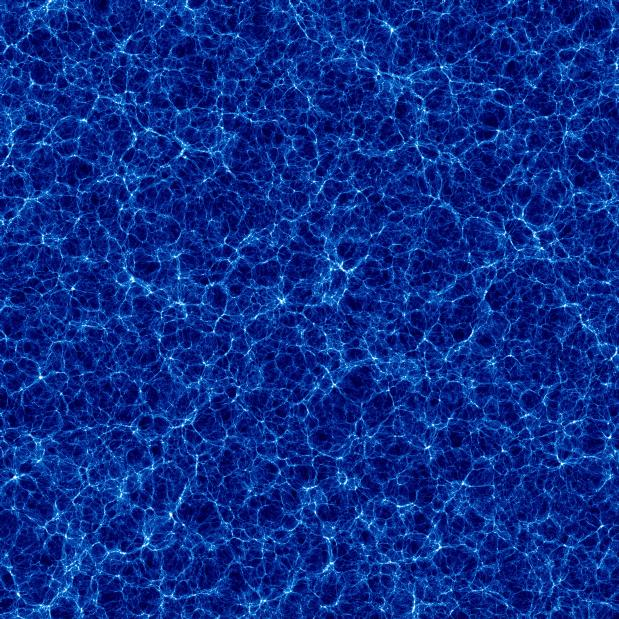
\includegraphics[width=4.2in]{Figures/thnucdmlowres.jpg}
}
  \frame{
    \frametitle{Differential clustering}
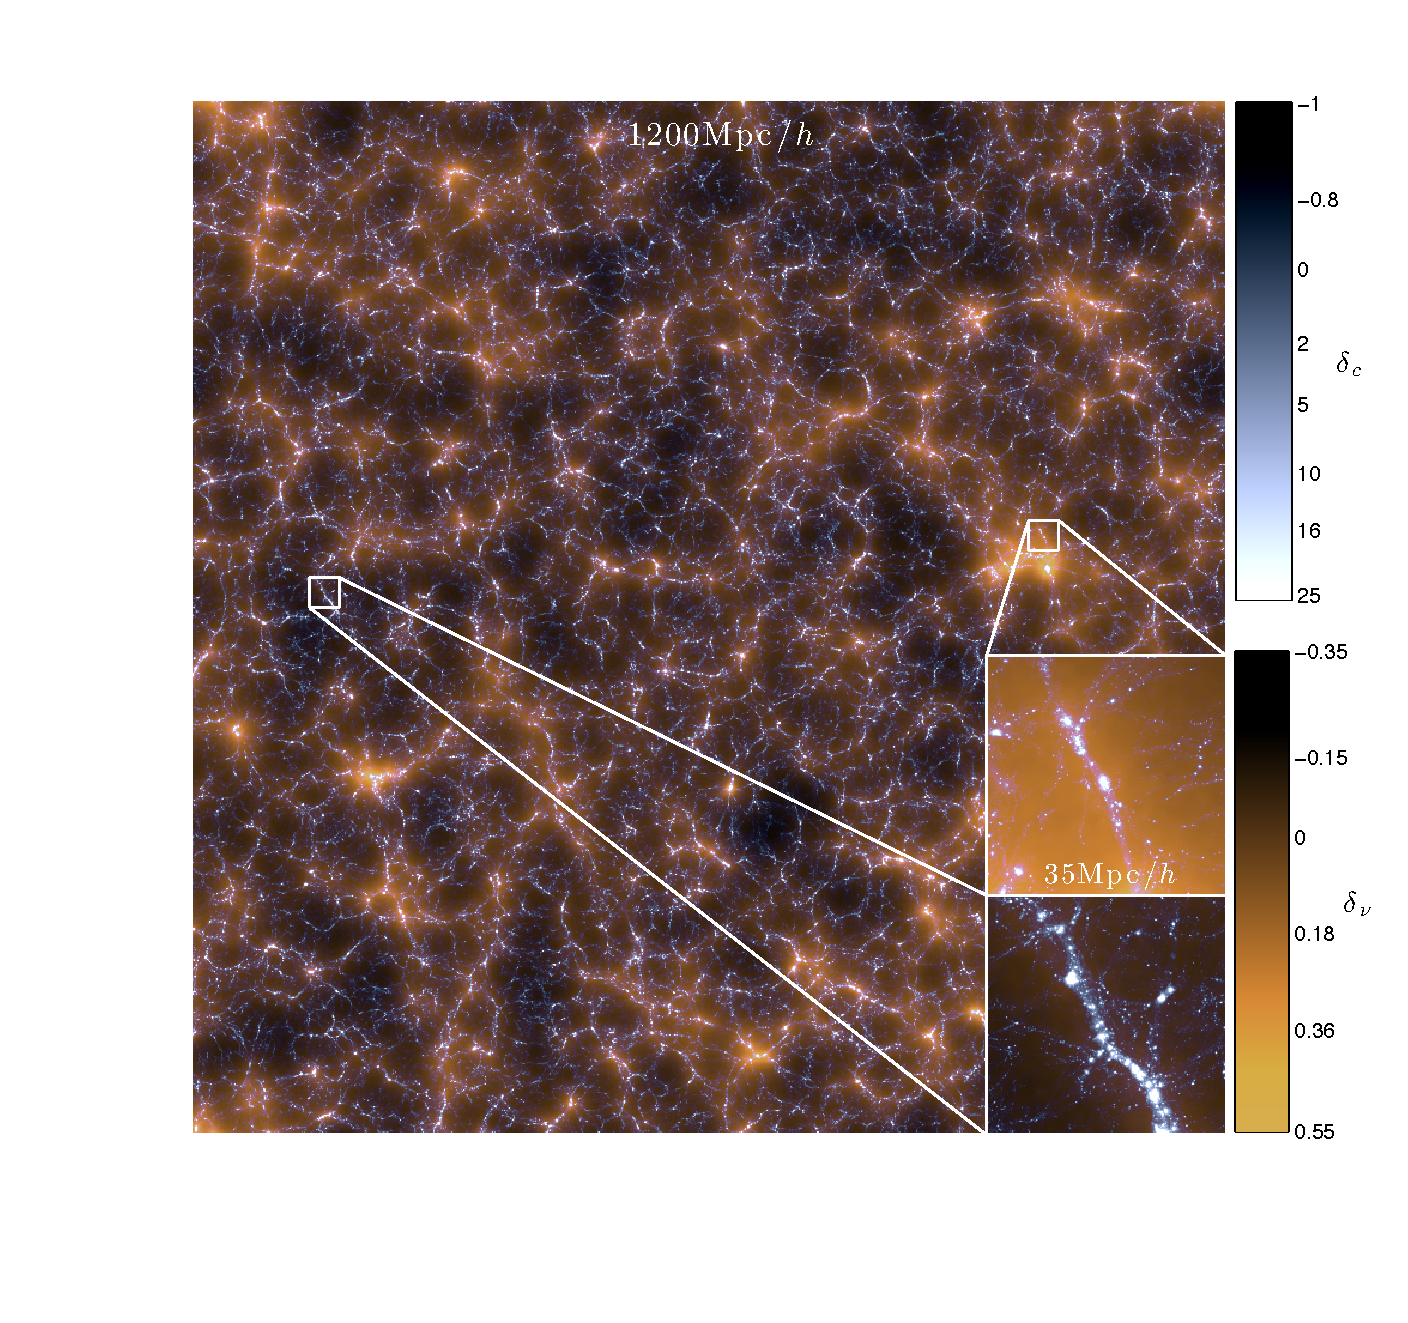
\includegraphics[width=3.5in]{Figures/cnudiff.pdf}
}
  \frame{
    \frametitle{Halo Reconstructed $\nu$ field}
%\vspace{0.5in} 
left: sim, right: wiener halo reconstructed
\vspace{-0.9in}
\hspace{-0.6in}
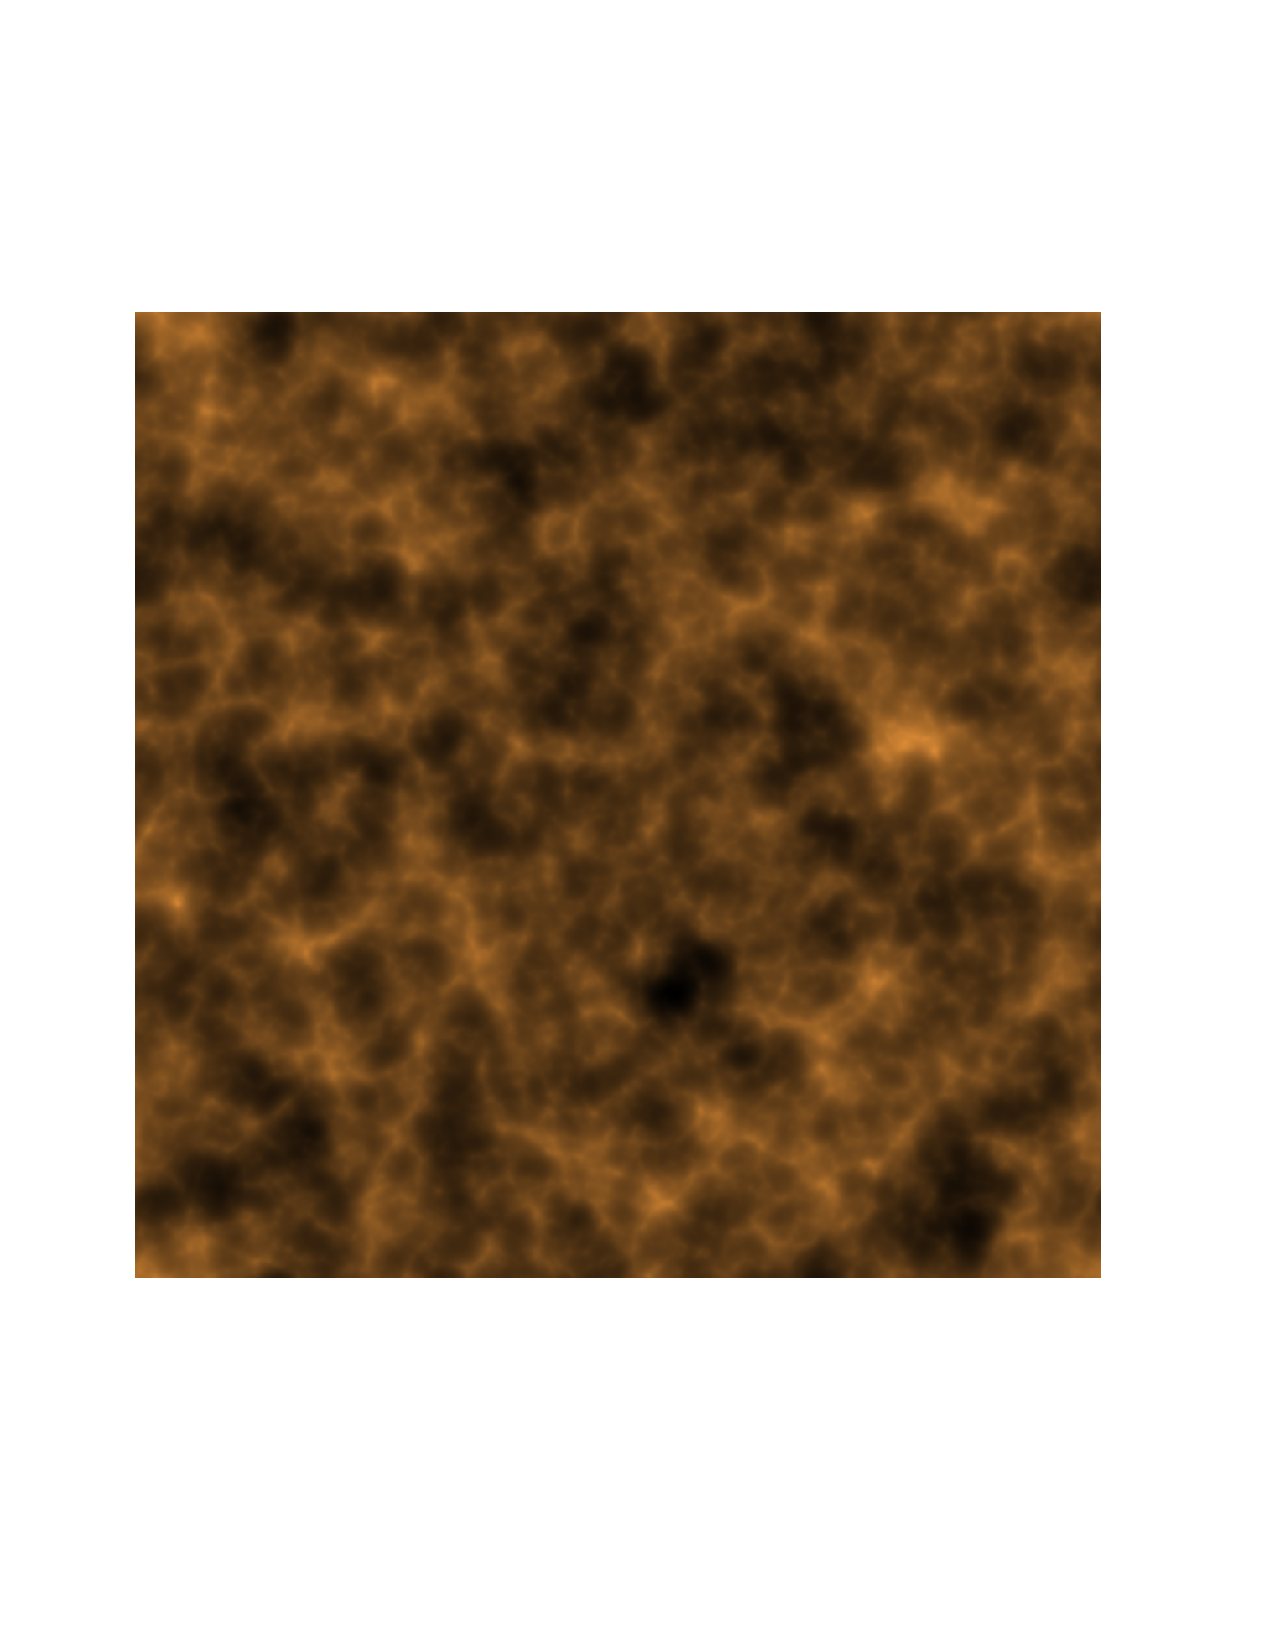
\includegraphics[width=2.7in]{Figures/delta_nu_reco_wien.pdf}
\hspace{-0.6in}\includegraphics[width=2.7in]{Figures/delta_nu_sim.pdf}
}
  \frame{
    \frametitle{\nu -Condensation}
\vspace{-1.0in}
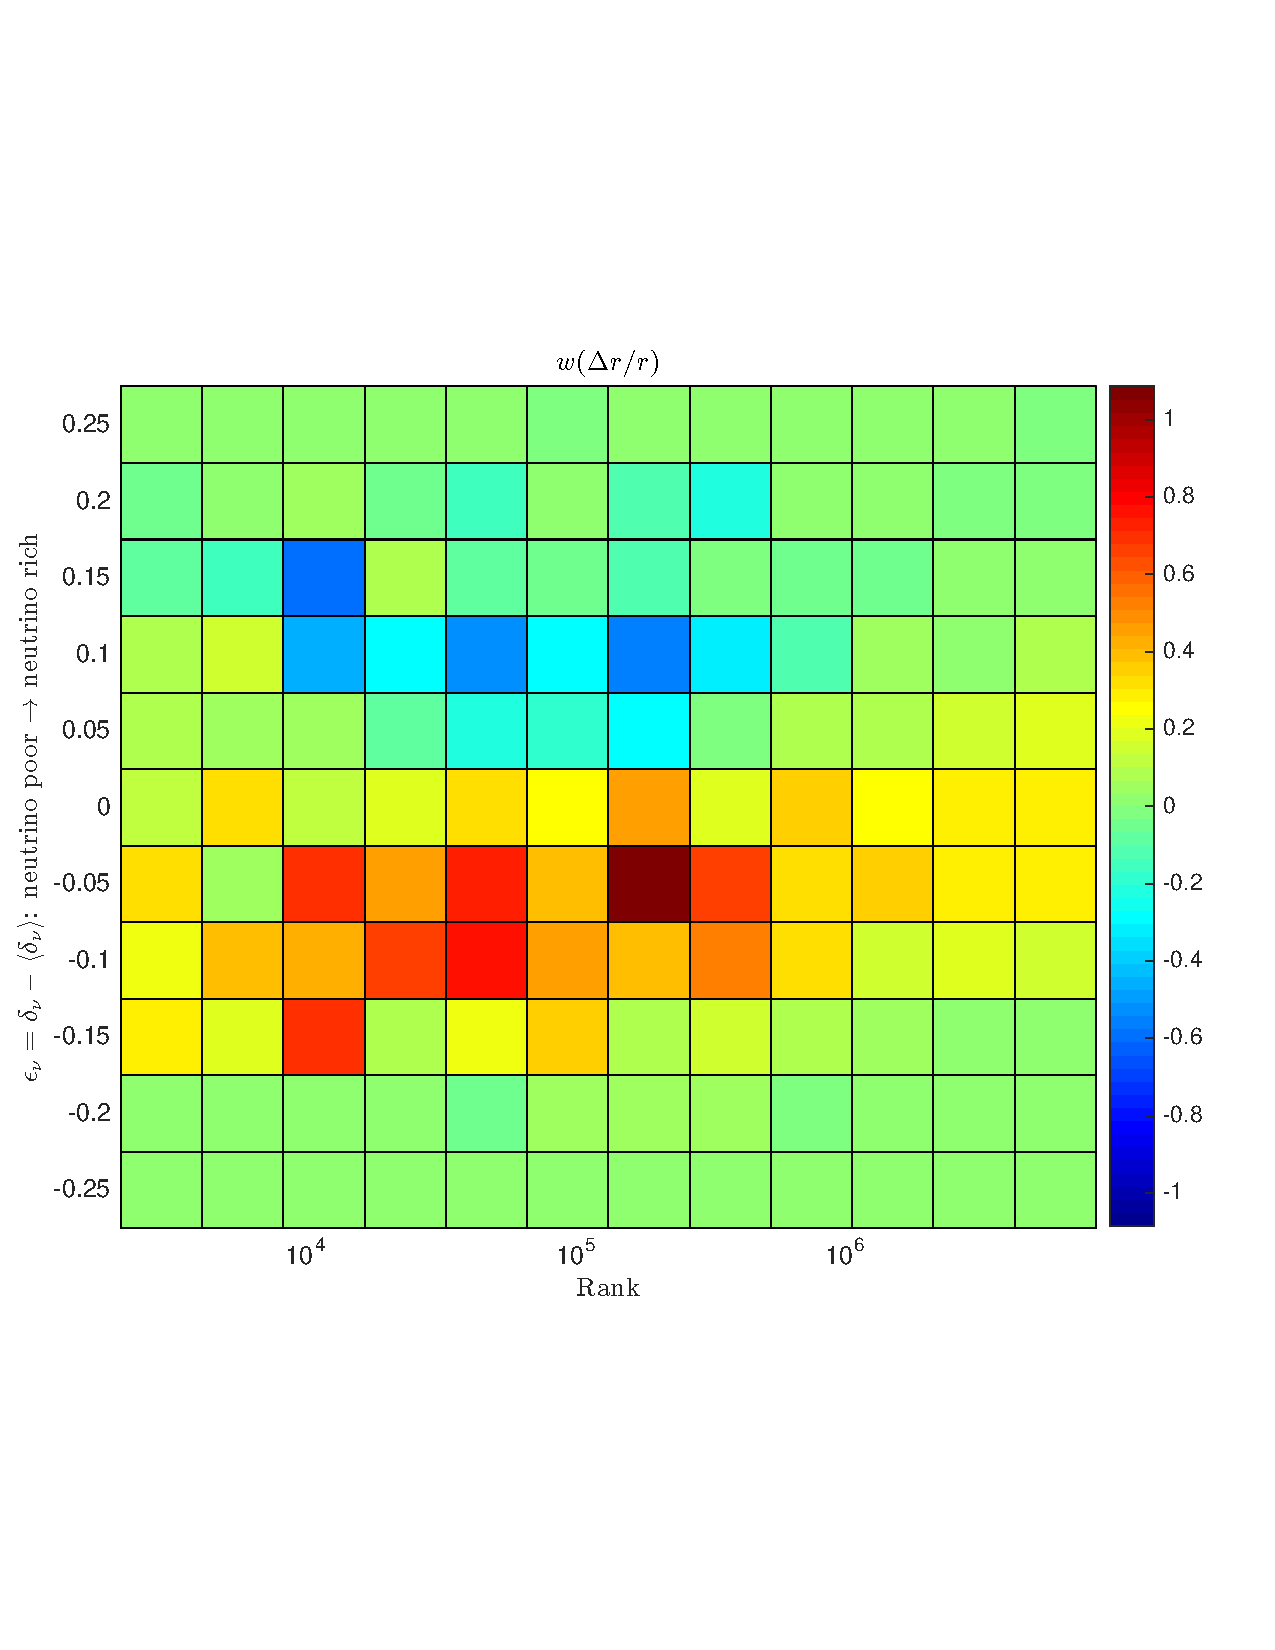
\includegraphics[width=4.0in]{Figures/color.pdf}
}
  \frame{
    \frametitle{\nu -bias}
\vspace{-1.0in}
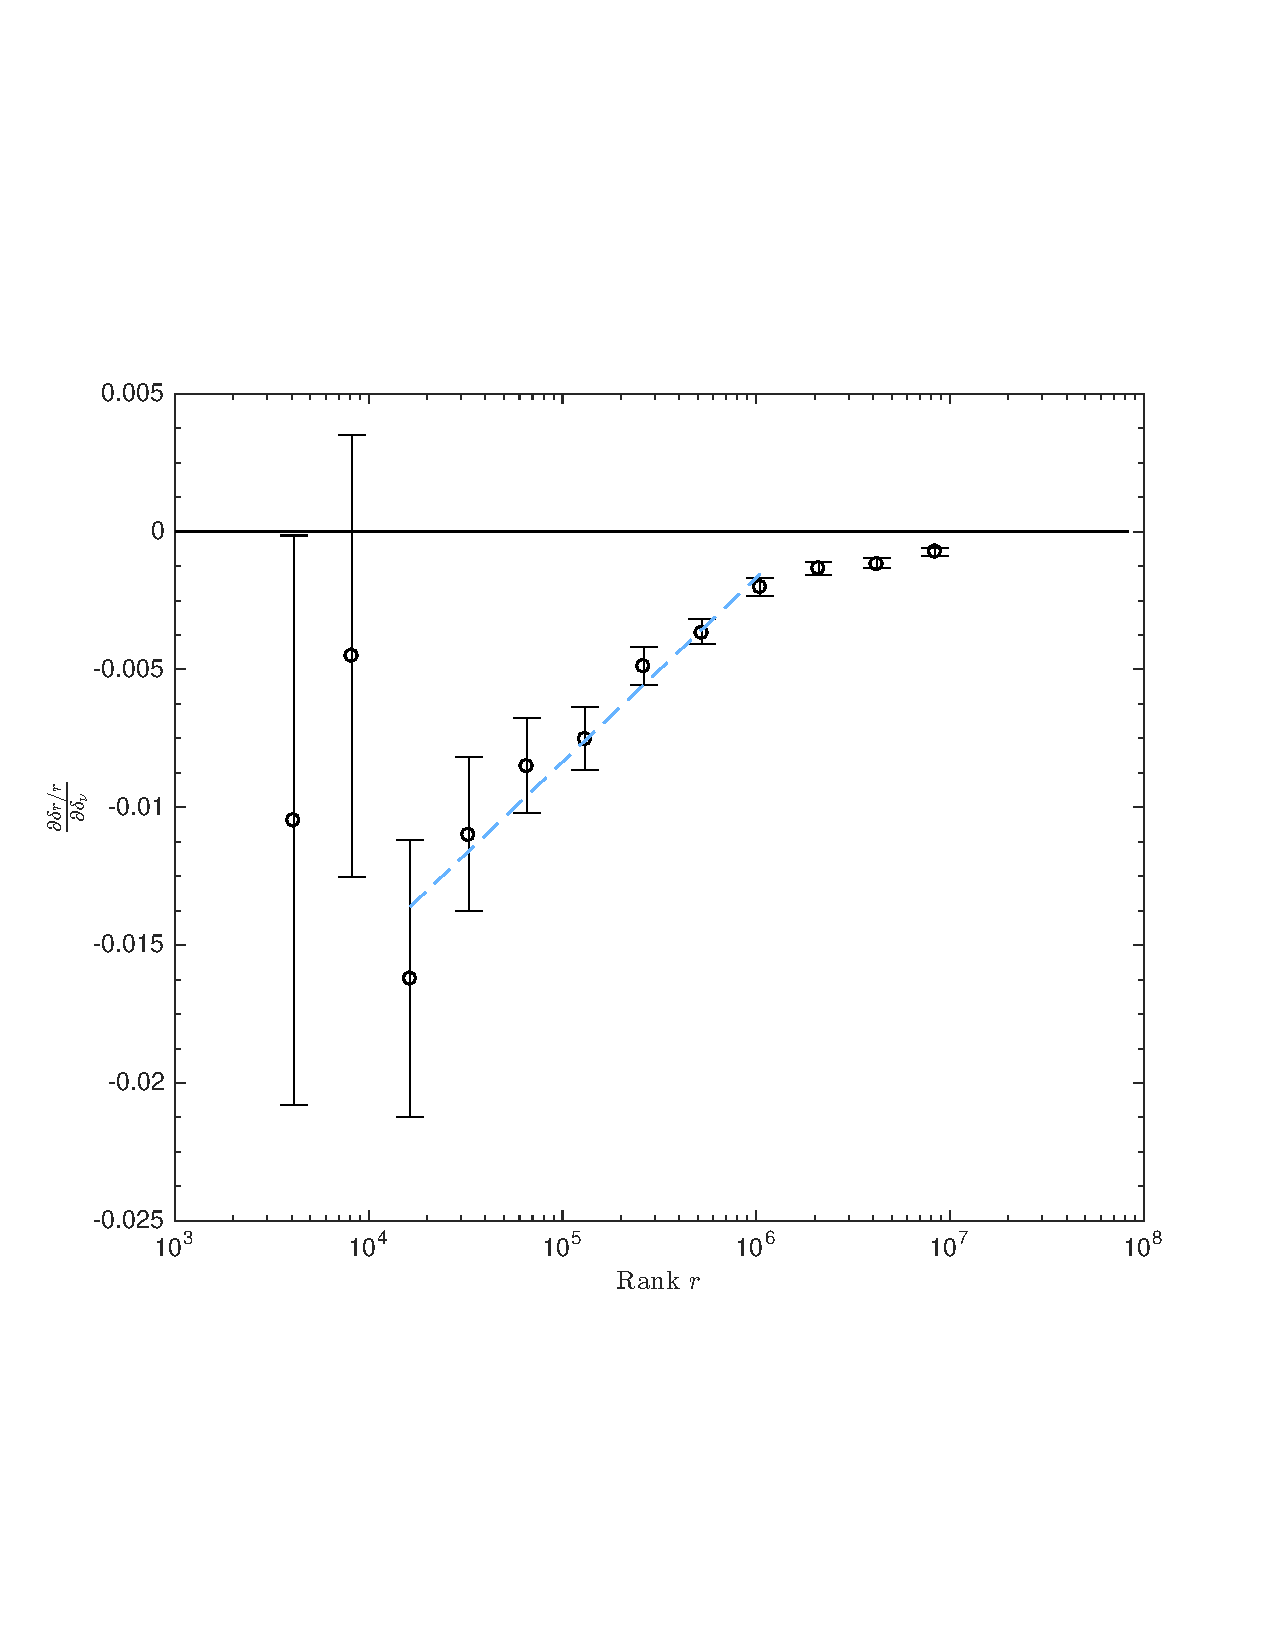
\includegraphics[width=4.0in]{Figures/slope_fit}
}
  \frame{
    \frametitle{Mass rank}
\vspace{-0.9in}
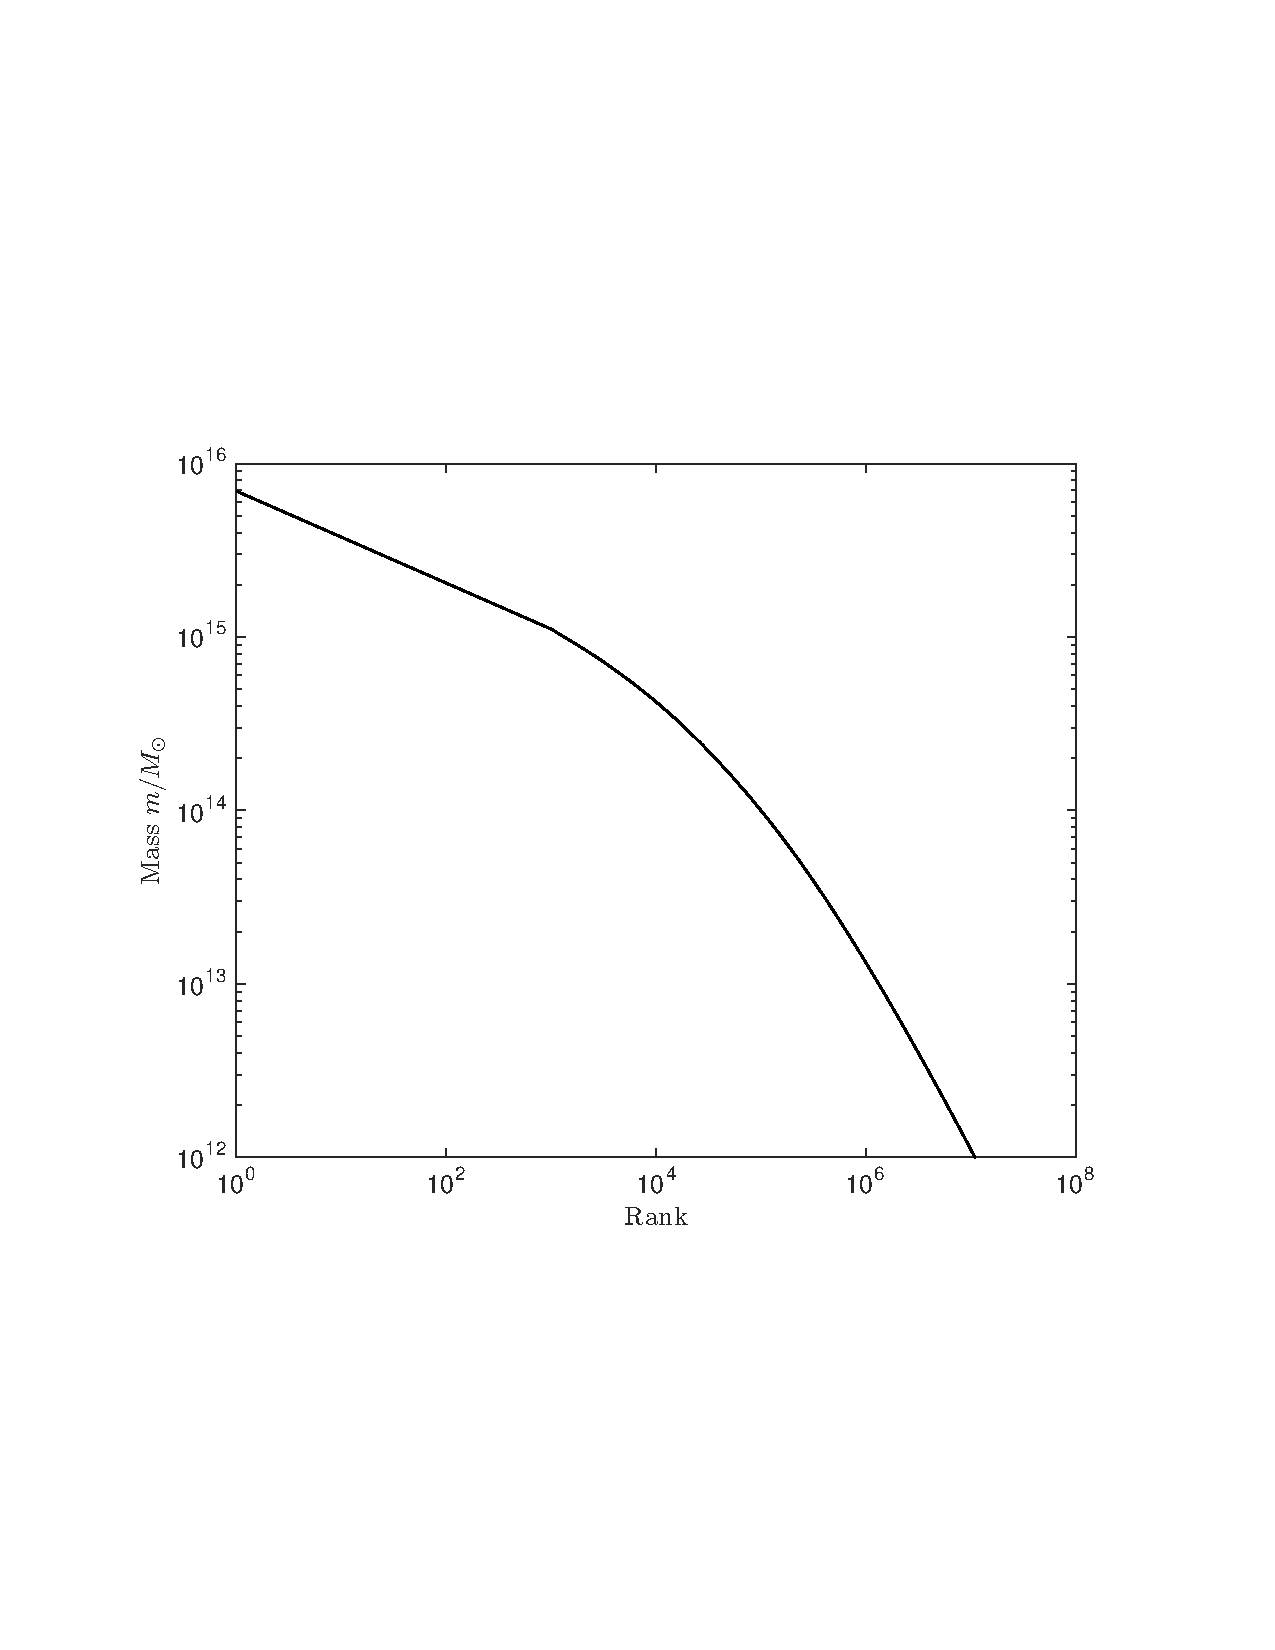
\includegraphics[width=4.0in]{Figures/HMF.pdf}
}
\end{document}
